\section{Experiments - outperforms state-of-the-art}
\begin{frame}{Experiments}
    \begin{itemize}
        \item 3 datasets (provided by Joachims) 
            \begin{itemize}
                \item Reuters CCAT (800K examples, 47k features)
                \item Covertype (581k examples, 54 features)
                \item Physics ArXiv (62k examples, 100k features)
            \end{itemize}
        \item 4 competing algorithms
            \begin{itemize}
                \item SVM-Perf (Joachims'06)
                \item SVM-light (Joachims)
                \item Norma (Kivinen, Smola, Williamson '02)
                \item Zhang'04 (stochastic gradient descent)
            \end{itemize}
    \end{itemize}
\end{frame}

\begin{frame}{Linear kernels}
\begin{table}[ht]
    \centering
    \begin{tabular}{l|l|l|l|l|l}
            \hline
            Dataset & Training & Testing & Features & Sparsity(\%) & $\lambda$ \\ \hline 
            astro-ph & 29,882 & 32,487 & 99,757 & 0.08 & $5\times 10^{-5}$ \\ 
            CCAT & 781,265 & 23,149 & 47,236 & 0.16 & $10^{-4}$ \\ 
            cov1 & 522,911 & 58,101 & 54 & 22.22 & $10^{-6}$ \\ \hline
        \end{tabular}
    \end{table}
\end{frame}

\begin{frame}{Linear kernels}
\begin{table}[ht]
    \centering
    \begin{tabular}{lllll}
            \hline
            Dataset & Pegasos & SDCA & SVM-Perf & LASVM \\ \hline 
            astro-ph & 0.04s(3.56\%) & 0.03s(3.49\%) & 0.1s(3.39\%) & 54s(3.65\%) \\ 
            CCAT & 0.16s(6.16\%) & 0.36s(6.57\%) & 3.6s(5.93\%) & $>$18000 s  \\ 
            cov1 & 0.32s(23.2\%) & 0.20s(22.9\%) & 4.2s(23.9\%) & 210s(23.8\%) \\ \hline
        \end{tabular}
    \end{table}
\end{frame}

\begin{frame}{Comparison of linear SVM optimizers}
    \begin{figure}[htbp]
        \centering
        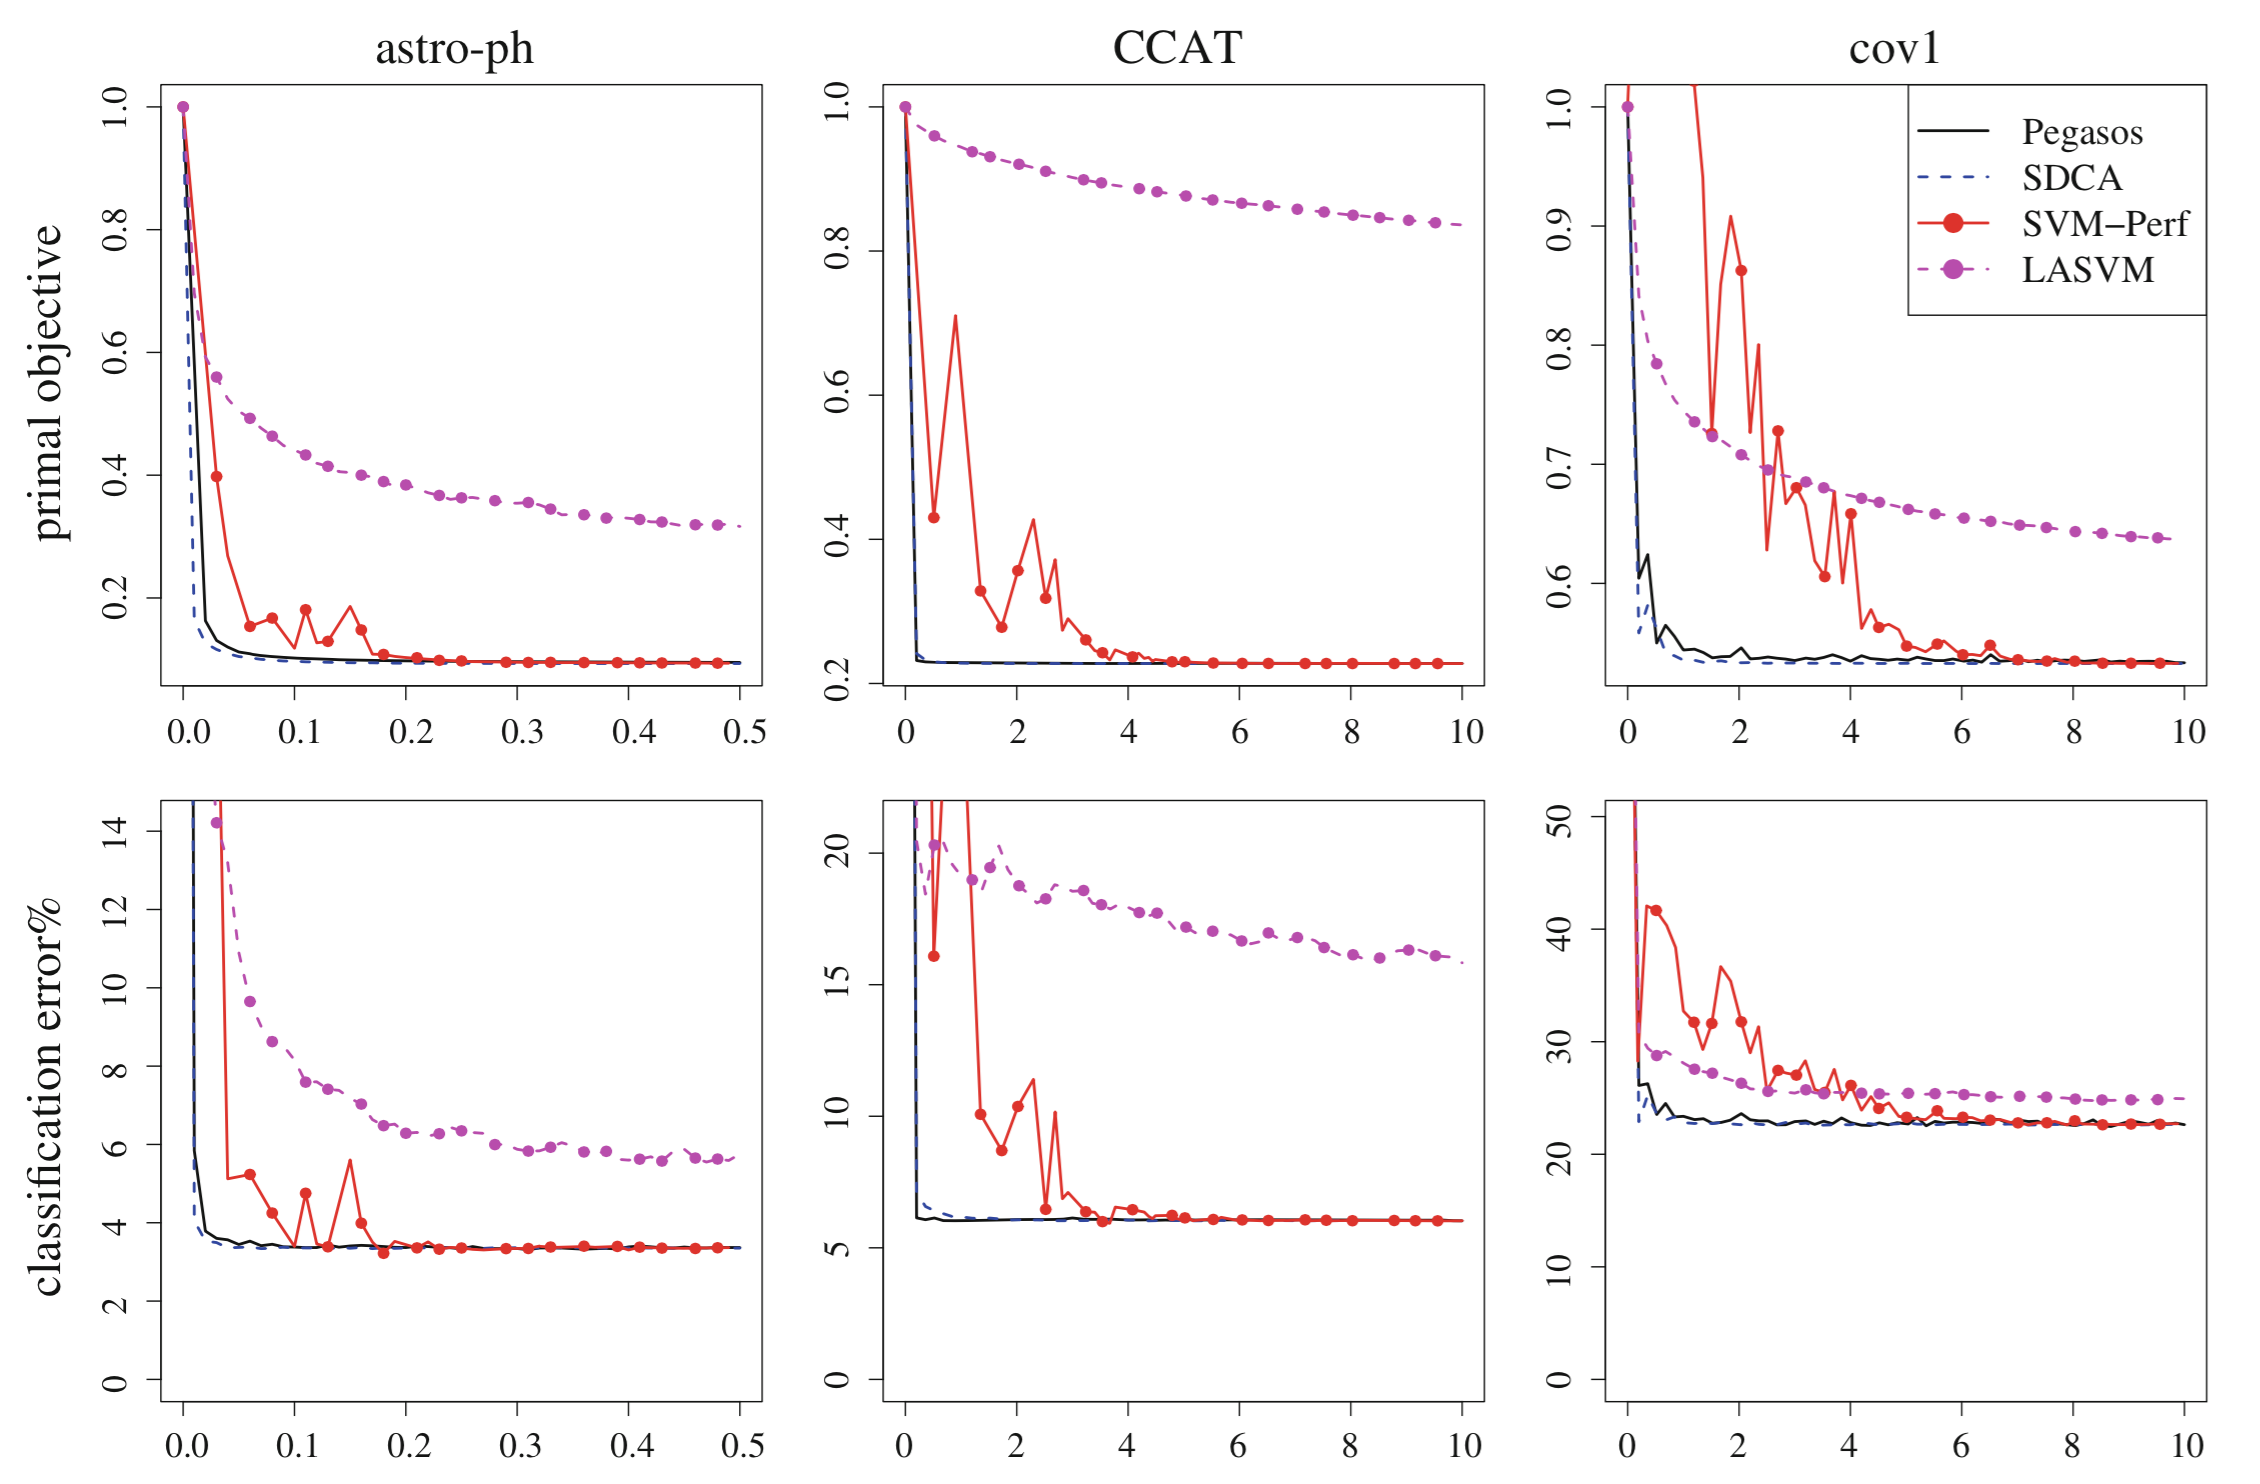
\includegraphics[height=0.7\textheight, width=\textwidth]{images/comp1.png}
    \end{figure}
\end{frame}

\begin{frame}{Effect of regularization parameter $\lambda$}
    \begin{figure}[htbp]
        \centering
        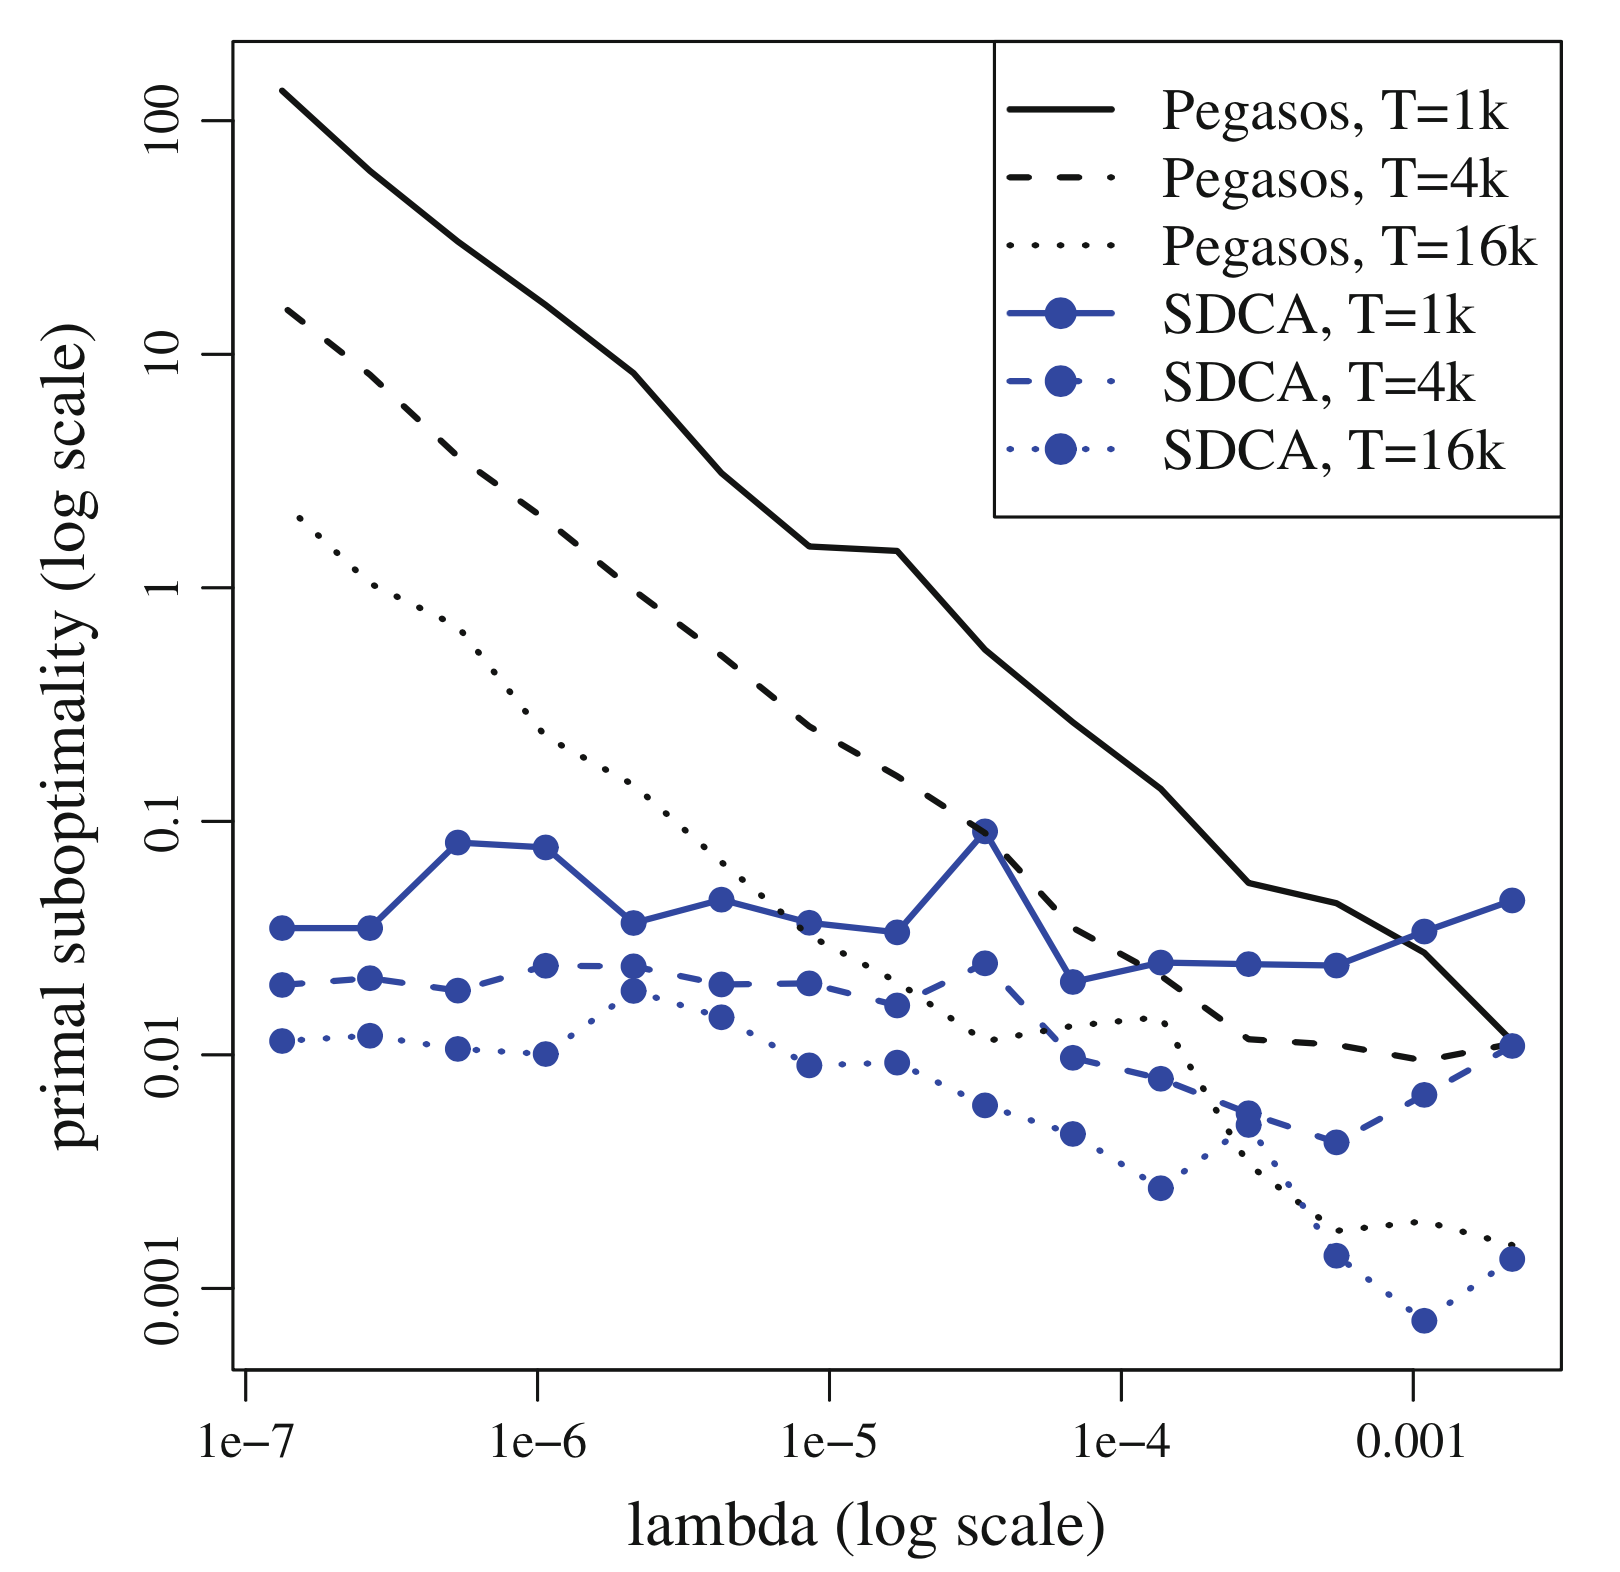
\includegraphics[height=0.7\textheight, width=0.7\textwidth]{images/comp_T.png}
    \end{figure}
\end{frame}

\begin{frame}{Experiments with the mini-batch variant}
    \begin{figure}[htbp]
        \centering
        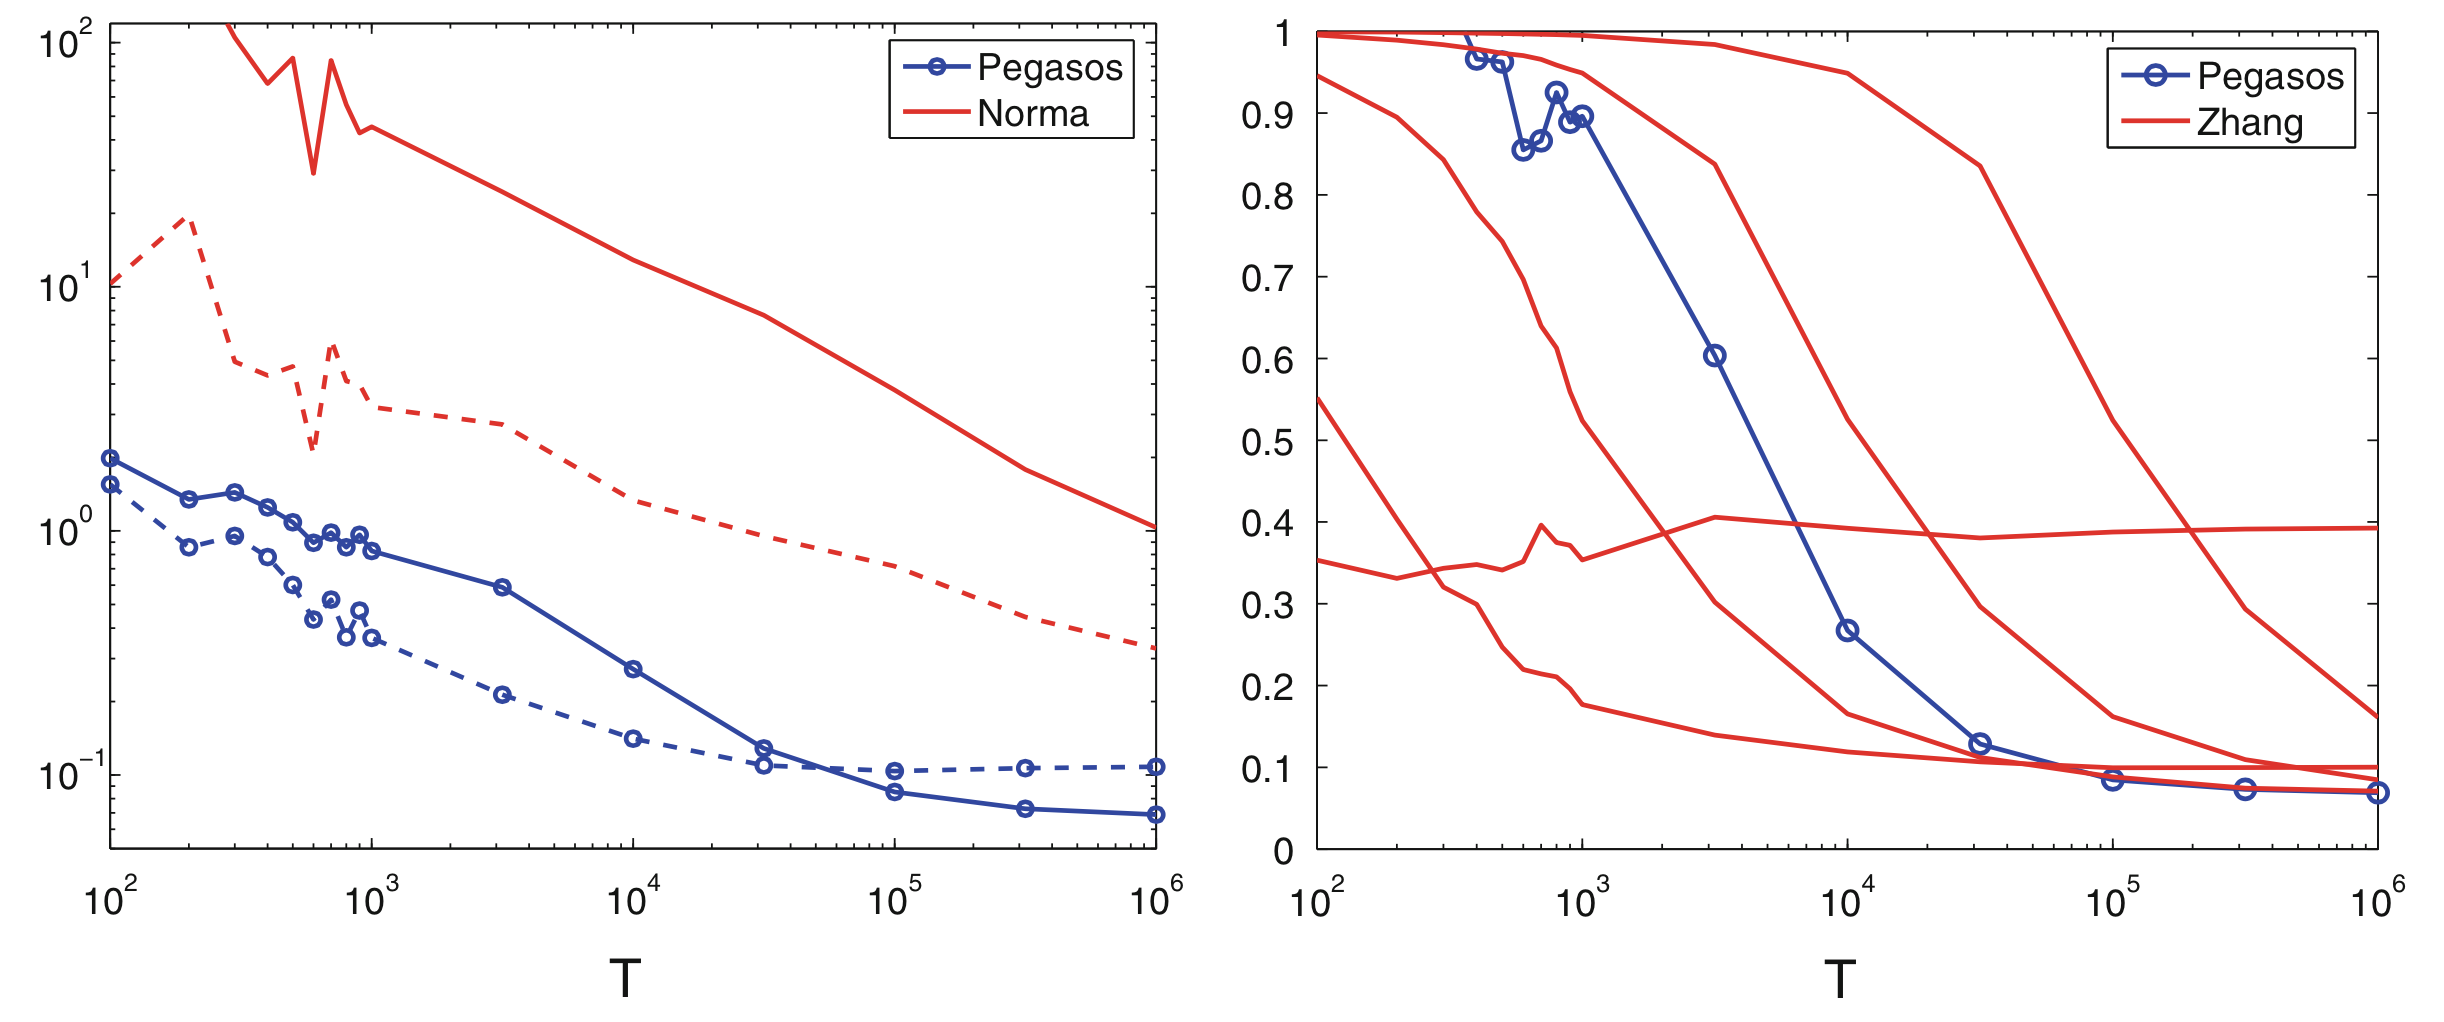
\includegraphics[height=0.7\textheight, width=\textwidth]{images/comp_k.png}
    \end{figure}
\end{frame}

\begin{frame}{Comparison of sampling procedures}
    \begin{figure}[htbp]
        \centering
        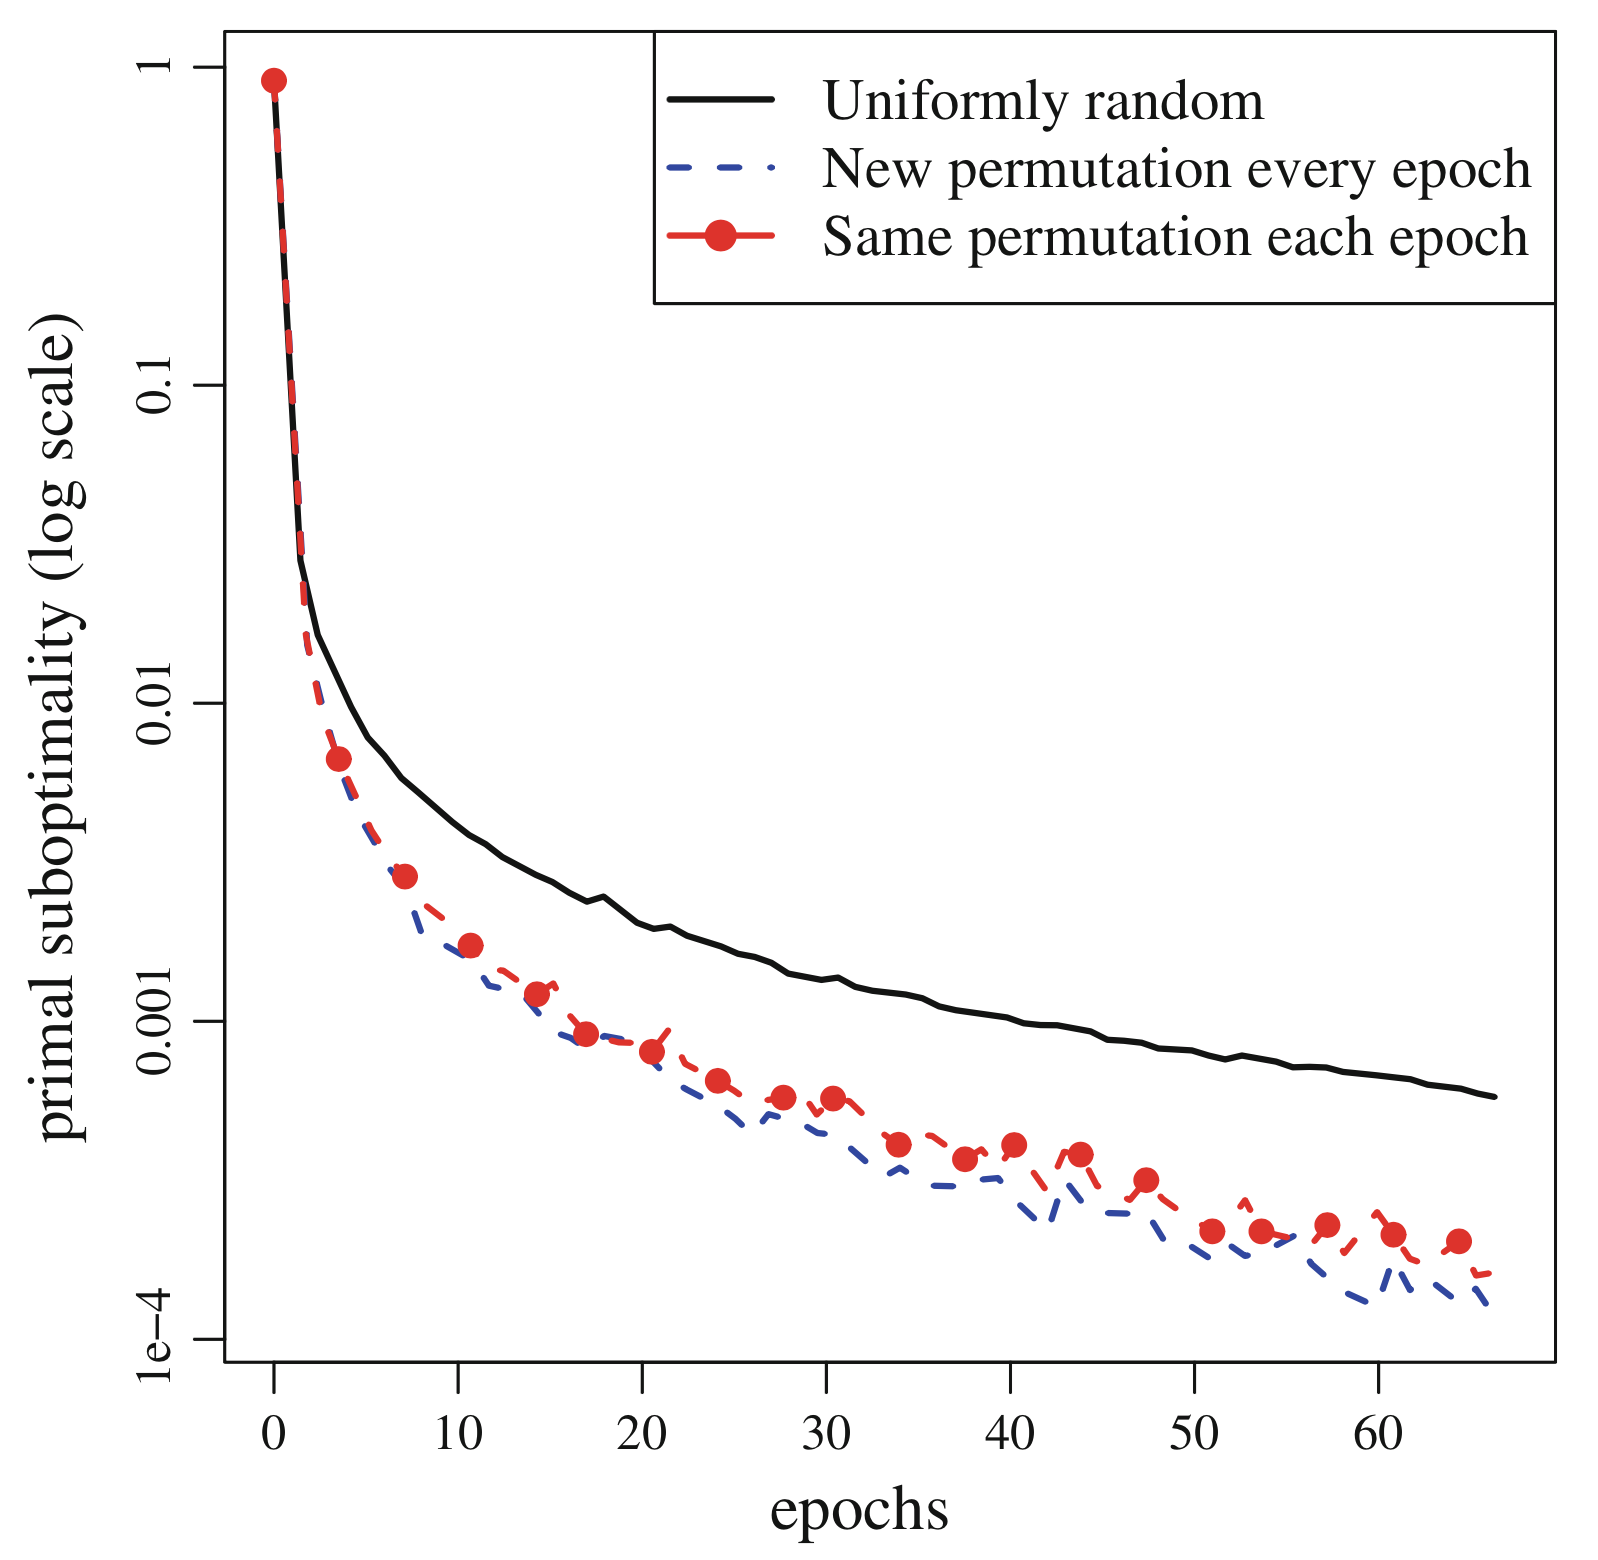
\includegraphics[height=0.7\textheight, width=0.7\textwidth]{images/epochs.png}
    \end{figure}
\end{frame}

\begin{frame}{Compare to Norma and Zhang (on Physics)}
    \begin{figure}[htbp]
        \centering
        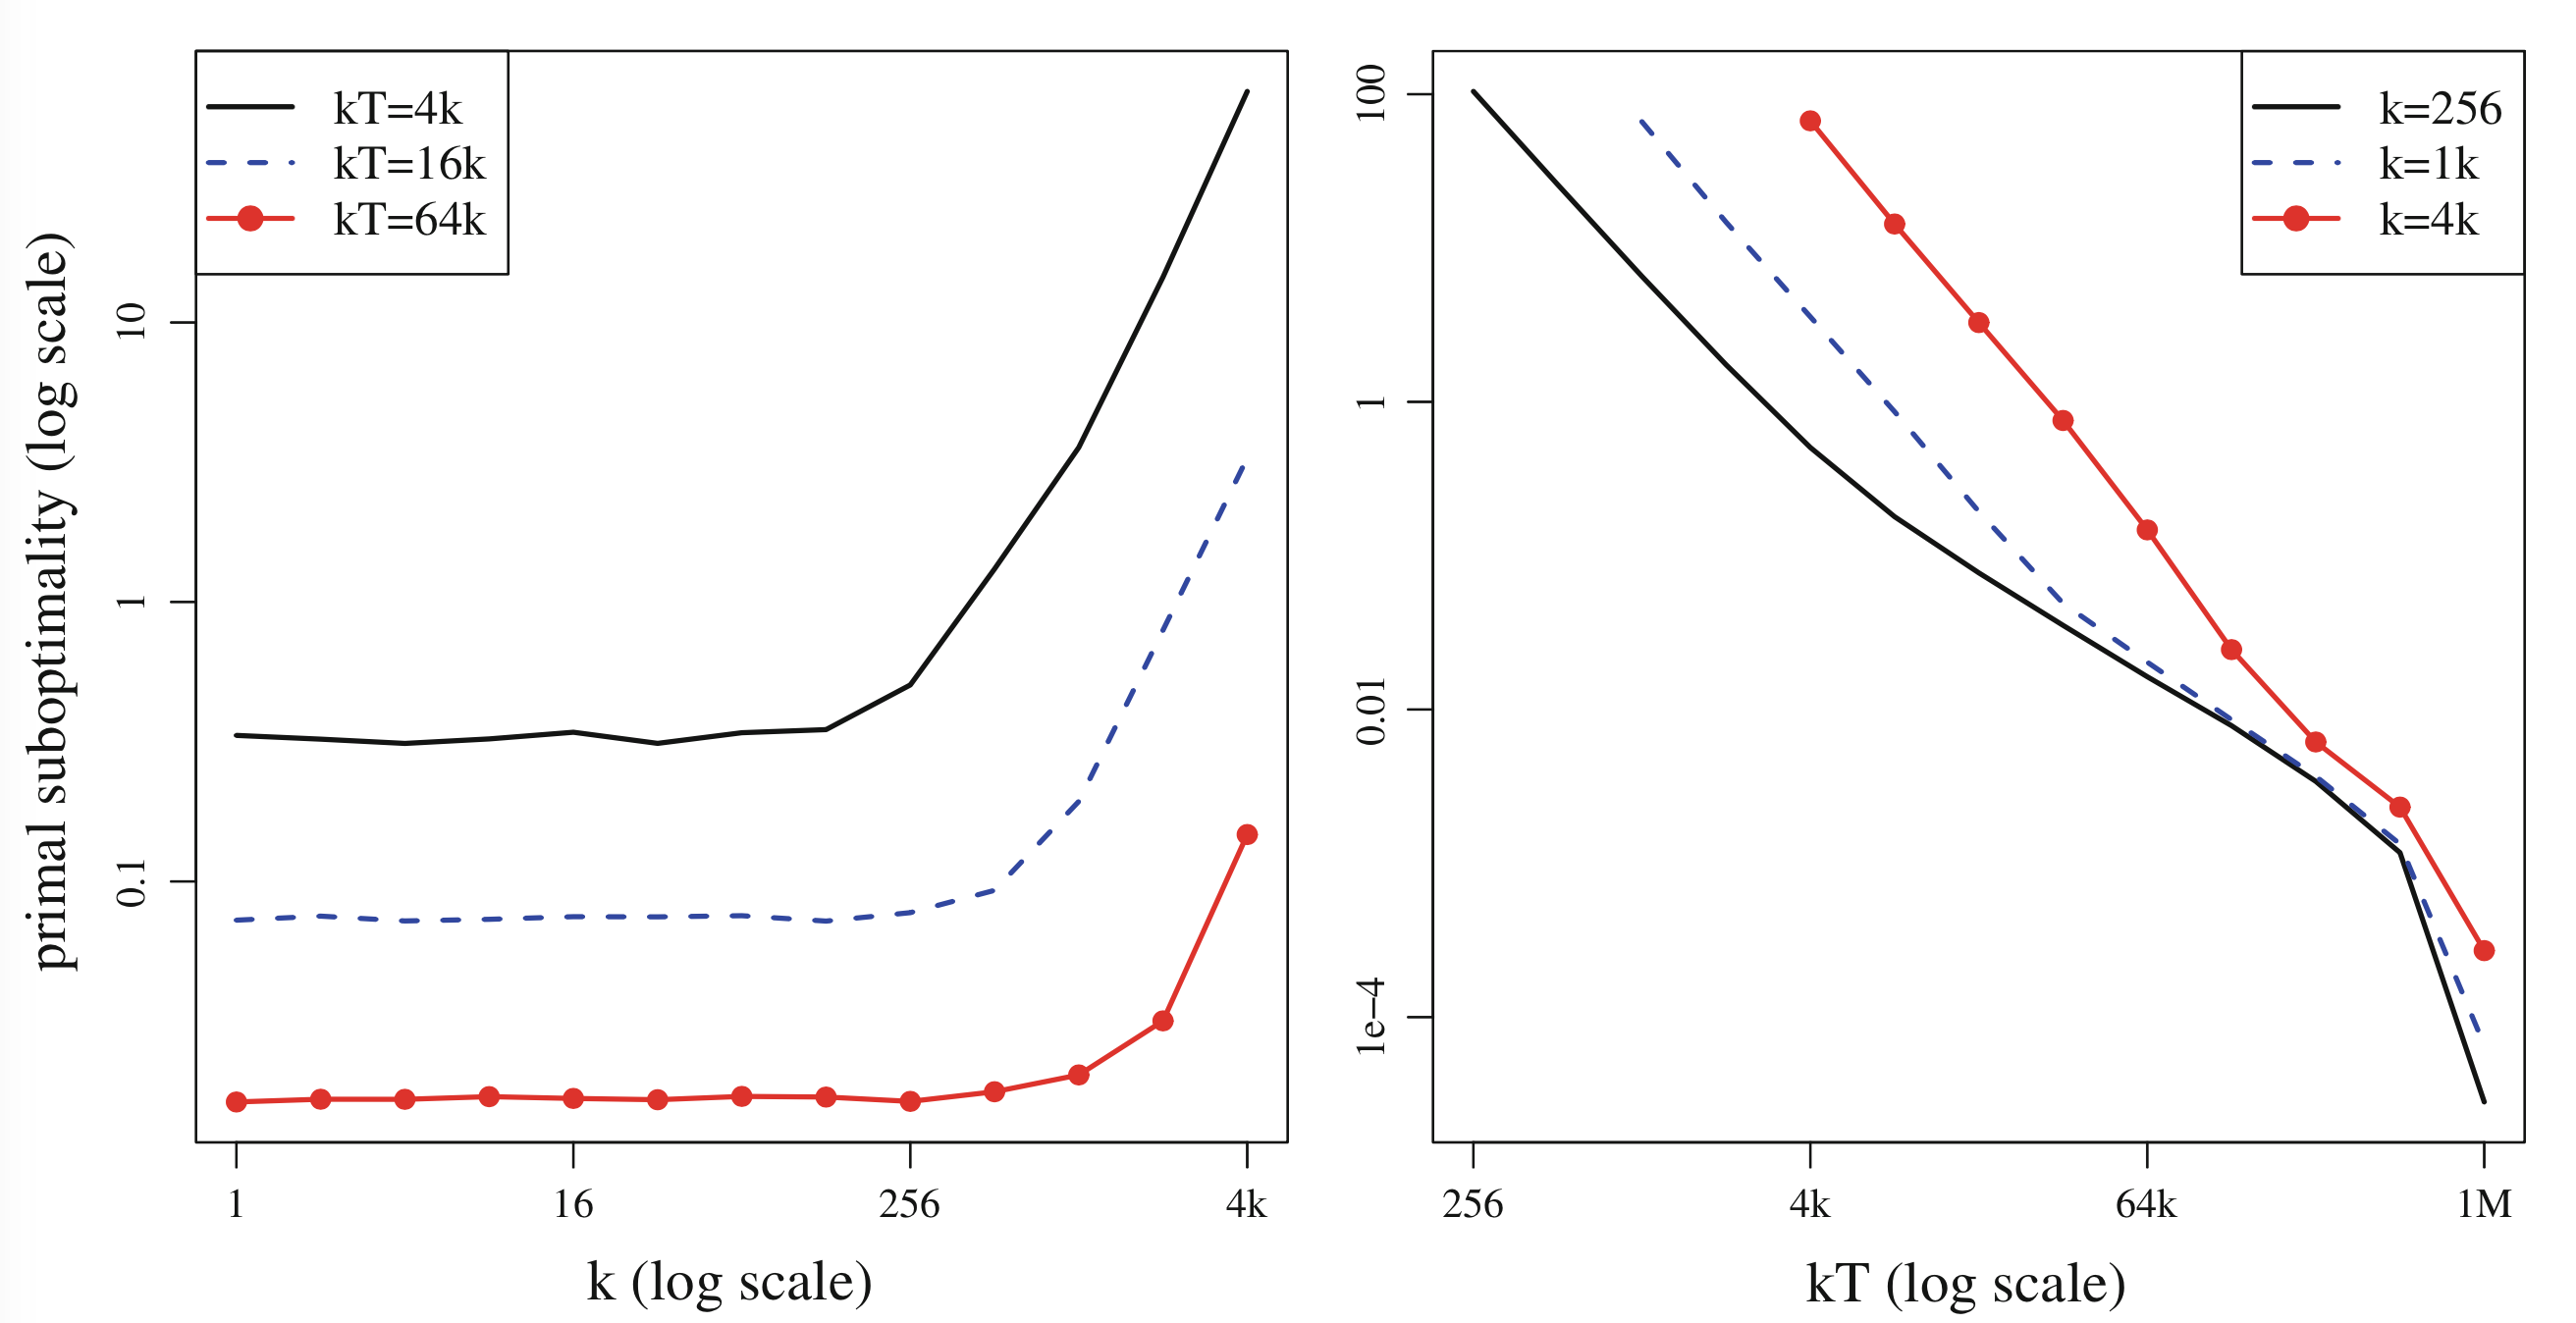
\includegraphics[height=0.7\textheight, width=\textwidth]{images/comp_nzh.png}
    \end{figure}
\end{frame}

\begin{frame}{Kernels}
    The basic Pegasos algorithm can easily be implemented using only kernel evaluations.
    \begin{itemize}
        \item For each t let $\mathbb{\alpha}_{t+1}\in R^n$ be the vector such that $\alpha_{t+1}[j]$ counts how many times example $j$ has been selected so far and we had a non-zero loss on it, namely, $\alpha_{t+1}[j]=\ |{t'\le t:i_{t'}=j\ \wedge\ y_j\langle \wv_{t'},\phi(\xv_j)\rangle < 1}|$.
        \item Represent $\wv_{t+1} = \frac{1}{\lambda t} \sum_{j=1}^{m} \alpha_{t+1}[j]y_j\phi(\xv_j)$
        \item {\color{green}Cons: overall runtime $\tilde{O}(md/(\lambda \epsilon))$}
    \end{itemize}
\end{frame}

\begin{comment}
\begin{frame}{Bias term}
    \begin{enumerate}
        \item Popular approach: increase dimension of $x$

            {\color{green}Cons: ``pay'' for $b$ in the regularization term}
        \item Define: $L(\wv) = \min_b \sum_{(\xv,y)\in S} [1-y(\langle \wv, \xv\rangle - b)]_+$
        \item Rewrite problem: $\min_{\wv} {\frac{\lambda}{2}\|\wv\|^2+g(\wv;S)}$ where $g(\wv;S)=\min_b \frac1m \sum_{(\xv,y)\in S} \left[1-y(\langle \wv, \xv\rangle + b)\right]_+$

        Calculate subgradients w.r.t $w$ and w.r.t $b$.

        \item Search $b$ in an outer loop

            {\color{green}Cons: evaluation time remain same as unbiased}
    \end{enumerate}
\end{frame}
\end{comment}

\begin{frame}{Discussion}
    \begin{itemize}
        \item Pegasos: Simple $\&$ Efficient solver for SVM
        \item Sample vs. computational complexity
            \begin{itemize}
                \item Sample complexity: How many examples do we need as a function of VC-dim($\lambda$), accuracy($\epsilon$), and confidence($\delta$)
                \item in Pegasos, we aim at analyzing computational complexity based on $\lambda$, $\epsilon$, $\delta$ (also in Bottou $\&$ Bousquet)
            \end{itemize}
        \item Finding argmin vs. calculating min: It seems that Pegasos finds the argmin more easily than it requires to calculate the min value
    \end{itemize}
\end{frame}

